\section{Поиск ассоциативных правил - общие понятия}
Задача поиска ассоциативных правил - задача "обучения без учителя". У нас есть объекты и признаки:
\begin{align*}
X & \text{ — пространство объектов;} \\
\mathcal{F} &= \{f_1, \ldots, f_n\}, \; f_j: X \rightarrow \{0, 1\} \text{ — бинарные признаки (принято называть item-ами);} \\
X^\ell &= \{x_1, \ldots, x_\ell\} \subseteq X \text{ — обучающая выборка.}
\end{align*}

Каждому подмножеству столбцов $\varphi \subseteq \mathcal{F}$ поставим в соотвествие конъюнкцию
\[
\varphi(x) = \bigwedge_{f \in \varphi} f(x), \quad x \in X.
\]

Если $\varphi(x) = 1$, то признаки из $\varphi$ "совместно встречаются" у $x$.

Частота встречаемости (поддержка, support) $\varphi$ в выборке $X^\ell$ - доля объектов обучающей выборки, на которых конъюнкция возвращает 1:
\[
\nu(\varphi) = \frac{1}{\ell} \sum_{i=1}^\ell \varphi(x_i).
\]

$\delta$ - минимальная поддержка (MinSupp), зафиксированный параметр. Если $\nu(\varphi) \geq \delta$, то «набор признаков $\varphi$ частый».

Мы собираемся искать все такие подмножества признаков, у которых $\nu(\varphi) \geq \delta$
\newline

\subsection{Определение ассоциативного правила}
\textbf{Определение}
Ассоциативное правило (association rule) $\varphi \rightarrow y$ — пара непересекающихся наборов $\varphi, y \subseteq \mathcal{F}$ таких, что:
\begin{enumerate}
    \item Наборы $\varphi$ и $y$ совместно часто встречаются,
    \[
    \nu(\varphi \cup y) \geq \delta;
    \]
    \item Во всех наборах, где встерчается $\varphi$, $y$ также должен встречаться достаточно много раз
    \[
    \nu(y \mid \varphi) \equiv \frac{\nu(\varphi \cup y)}{\nu(\varphi)} \geq \chi.
    \]


\end{enumerate}

$\nu(y \mid \varphi)$ — значимость правила.
Параметр $\delta$ — минимальная поддержка, MinSupp.
Параметр $\chi$ — минимальная значимость, MinConf.

\subsection{Примеры}
\textbf{Пример: анализ рыночных корзин (market basket analysis) [1993]}

Одним из применений является такая задача: мы хотим выяснить, насколько часто товары покупаются вместе (например, чтобы разместить эти товары на соседних стеллажах для увеличения прибыли).

\textit{Признаки} — товары (предметы, items)

\textit{Объекты} — чеки (транзакции)

\[ f_j(x_i) = 1 \] 
в \( i \)-м чеке зафиксирована покупка \( j \)-го товара.

\textbf{Пример}: «если куплен хлеб \(\varphi\), то будет куплено и молоко \(y\) с вероятностью \(\nu(y \mid \varphi) = 60\%\); причём оба товара покупаются совместно с вероятностью \(\nu(\varphi \cup y) = 2\%\)».

\textbf{Цели анализа:}
- оптимизировать размещение товаров на полках,
- формировать персональные рекомендации,
- планировать рекламные кампании (промо-акции),
- более эффективно управлять ценами и ассортиментом.
\newline
\newline
\textbf{Пример 2: выявление тематики в коллекциях текстовых документов}

\textit{Признаки} — термины (отдельные слова или выражения)

\textit{Объекты} — текстовые документы

\[ f_j(x_i) = 1 \]
в \( i \)-м тексте (часто) употребляется \( j \)-й термин.

\textit{Тема} — это совокупность терминов, совместно встречающихся в узком подмножестве документов, то есть \textit{частый набор}.

\textbf{Недостаток}: слишком жёсткое требование, чтобы в тексте встречались \textit{все} слова темы. Вероятностные модели адекватнее.

\subsection{Аналогия с логической закономерностью}
Определение ассоциативных правил похоже на определение логической закономерности (кроме того, что здесь нет ответов):
\newline
\textbf{Определение}
\newline
Предикат \(\varphi(x)\) — логическая \(\varepsilon, \delta\)-закономерность класса \(c \in Y\)

\[
D_c(\varphi, X^\ell) = \frac{p_c(\varphi)}{\ell} \geq \delta;
\]
\[
E_c(\varphi, X^\ell) = \frac{n_c(\varphi)}{p_c(\varphi) + n_c(\varphi)} \leq \varepsilon,
\]

\[
p_c(\varphi) = \#\{x_i : \varphi(x_i) = 1 \land y(x_i) = c\} \quad \text{— примеры класса } c;
\]
\[
n_c(\varphi) = \#\{x_i : \varphi(x_i) = 1 \land y(x_i) \neq c\} \quad \text{— примеры класса }\overline{c}.
\]

Для «\(\varphi \rightarrow y\)» возьмём целевой признак \(y(x) = \bigwedge_{f \in y} f(x)\). Тогда

\[
\nu(\varphi \cup y) \equiv D_1(\varphi) \geq \delta;
\]
\[
\frac{\nu(\varphi \cup y)}{\nu(\varphi)} \equiv 1 - E_1(\varphi) \geq 1 - \varepsilon \equiv \chi.
\]

Получается, что различия двух определений чисто терминологические.
\subsection{Свойство антимонотонности}
Поскольку \(\varphi(x) = \bigwedge_{f \in \varphi} f(x)\) — конъюнкция, имеет место

\textbf{Свойство антимонотонности:}
для любых \(\psi, \varphi \subseteq \mathcal{F}\) из \(\varphi \subseteq \psi\) следует \(\nu(\varphi) \geq \nu(\psi)\) (eсли объединить 2 признака, то поддержка может только уменьшиться)

Следствия:
\begin{enumerate}
    \item если \(\psi\) частый, то все его подмножества \(\varphi \subseteq \psi\) частые.
    \item если \(\varphi\) не частый, то все наборы \(\psi \supseteq \varphi\) также не частые.
    \item \(\nu(\varphi \cup \psi) \leq \nu(\varphi)\) для любых \(\varphi, \psi\).
\end{enumerate}

Два этапа поиска ассоциативных правил:
\begin{enumerate}
    \item поиск частых наборов (многократный просмотр транзакционной базы данных)
    \item выделение ассоциативных правил из частого набора (разделить на части посылка-следствие в оперативной памяти)
\end{enumerate}

\subsection{Задачи}

\textbf{Задача 1.}

В магазине проводятся продажи нескольких товаров: хлеб, молоко, сыр и яйца. По данным транзакций было обнаружено, что хлеб и молоко покупаются вместе с частотой $15\%$, а самому хлебу принадлежит частота $30\%$. Определите значимость правила: «если куплен хлеб, то куплено и молоко».
\newline
\textbf{Решение.}

Для оценки значимости правила «если куплен хлеб, то куплено и молоко», используем показатель \(\text{confidence}\), который определяется как:
\[
\text{confidence}(\text{хлеб} \rightarrow \text{молоко}) = \frac{\nu(\text{хлеб} \cup \text{молоко})}{\nu(\text{хлеб})}
\]

Подставим известные значения:
\[
\text{confidence} = \frac{0.15}{0.30} = 0.5
\]

Значение $0.5$ означает, что в $50\%$ случаев, когда покупают хлеб, также покупают молоко.
\newline
\textbf{Задача 2.}

Придумайте примеры из реальной где еще может быть полезен поиск ассоциативных правил.
\newline
\textbf{Решение.}

Компания Walmart использовала ассоциативные правила для анализа покупок своих клиентов и обнаружила, что во время ураганов продажи капустного пива значительно возрастали вместе с продажами скотчей. Это позволило им оптимизировать размещение этих товаров в магазинах и создать более эффективные маркетинговые кампании.

Ассоциативные правила активно используются в системе рекомендаций Amazon, которая предлагает клиентам такие товары, как книги, основанные на покупках других клиентов с похожими интересами. Например, если покупатели, которые купили книгу Властелин колец, также часто покупают Хоббит, это правило будет использоваться для рекомендации.

Банк HSBC применяет ассоциативные правила для выявления необычных паттернов транзакций, которые могут указывать на мошенническую активность. Например, если клиент обычно не делает крупных межгосударственных переводов, внезапная такая операция может быть помечена для дальнейшего расследования.

Компания Ford применяет ассоциативные правила для анализа данных о сборочных процессах, что помогает выявлять корреляции между использованием определенных компонентов и дефектами в конечных продуктах. Эти данные используются для улучшения процессов контроля качества.
\newline
\textbf{Задача 3.}

Как применять методы ассоциативных правил к данным, содержащим не только категориальные, но и количественные или непрерывные значения (например, количество купленных единиц товара, цена, вес)? Какие техники дискретизации или адаптации алгоритмов могут быть использованы для обработки таких данных, и как это повлияет на интерпретацию результатов?
\newline
\textbf{Решение.}

Для того чтобы применять ассоциативный анализ к непрерывным или количественным данным, их необходимо преобразовать в категориальную форму. Это достигается с помощью дискретизации — процесса разделения непрерывного диапазона значений на конечное число бинов, каждому из которых присваивается категория. После дискретизации непрерывных данных их можно представить в виде бинарных атрибутов, что необходимо для классических алгоритмов ассоциативных правил.

\section{Алгоритм FP-Growth}
Алгоритм FP-Growth был опубликован в 2005 году Кристианом Боргельтом, и до сих пор является передовым в поиске ассоциативных правил. Алгоритм APriory, работает за $O(nl\cdot 2^k)$, где $n$ - это число признаков, $l$ - число записей в базе, а $k$ - максимальный размер ассоциативного правила. В то же время FP-Growth работает за $O(nl + f(k, n))$.

Идея этого алгоритма лежит в создании бора всех наборов $\varphi$, который будет хранить всю информацию о частотах встречаемости наборов, благодаря чему нам не придётся каждый раз пробегать всю базу с целью подсчёта $\nu(\varphi)$
\newline\newline
Алгоритм состоит из двух этапов:
\begin{enumerate}
    \item Построение FP-дерева
    \item Построение списка ассоциативных правил
\end{enumerate}

\subsection{Построение FP-дерева}

\begin{figure}[h]
    \centering
    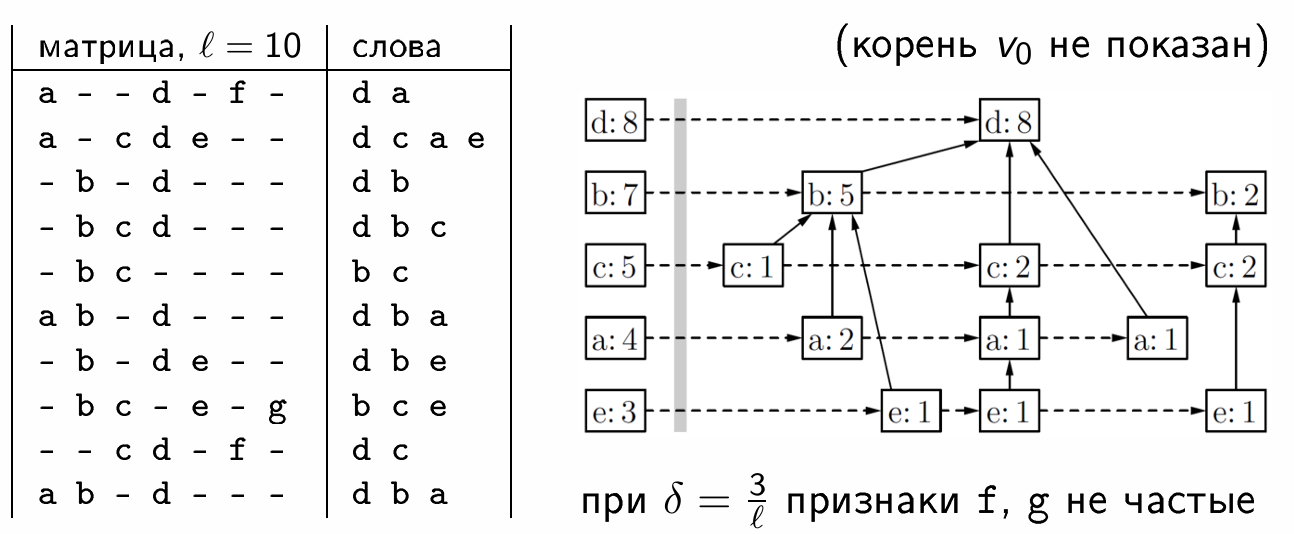
\includegraphics[width=0.8\linewidth]{chapters/rules/images/fp-tree-example.png}
    \caption{Пример FP-дерева}
\end{figure}

Первым делом упорядочим все признаки $f \in \mathcal{F}: \nu(f) \geq \delta$ по убыванию $\nu(f)$, их порядок будет соответствовать уровням вершин дерева (это не глубины!). Будем последовательно перебирать транзакции из базы. Будем хранить бор (FP-дерево), в каждой вершине $v$ которого будут храниться: 
\begin{enumerate}
    \item Признак $f_v \in \mathcal{F}$
    \item Множество дочерних вершин $S_v$
    \item Счетчик $c_v = \nu(\phi_v)$, где $\phi_v$ - набор состоящий из признаков соответствующих пути от корня до данной вершины. По сути этот счетчик равен количеству строк из базы, распознаваемых данной вершиной.
\end{enumerate}

Пусть для текущей транзакции $i$ положительны признаки из множества $F_i = \{f \in \mathcal{F}: f(x_i) = 1 \}$, упорядочим их по убыванию $\nu(f)$, получим строку $R_i$, начнем распознавать её бором. Если её нет в боре, создадим недостающие вершины, проинициализировав счетчики $c_{v_i} = 0$ в новых вершинах. Добавим 1 к счетчикам $c_v$ вершин, которые лежат на пути от корня, соответствующем $R_i$.

\begin{figure}[h]
    \centering
    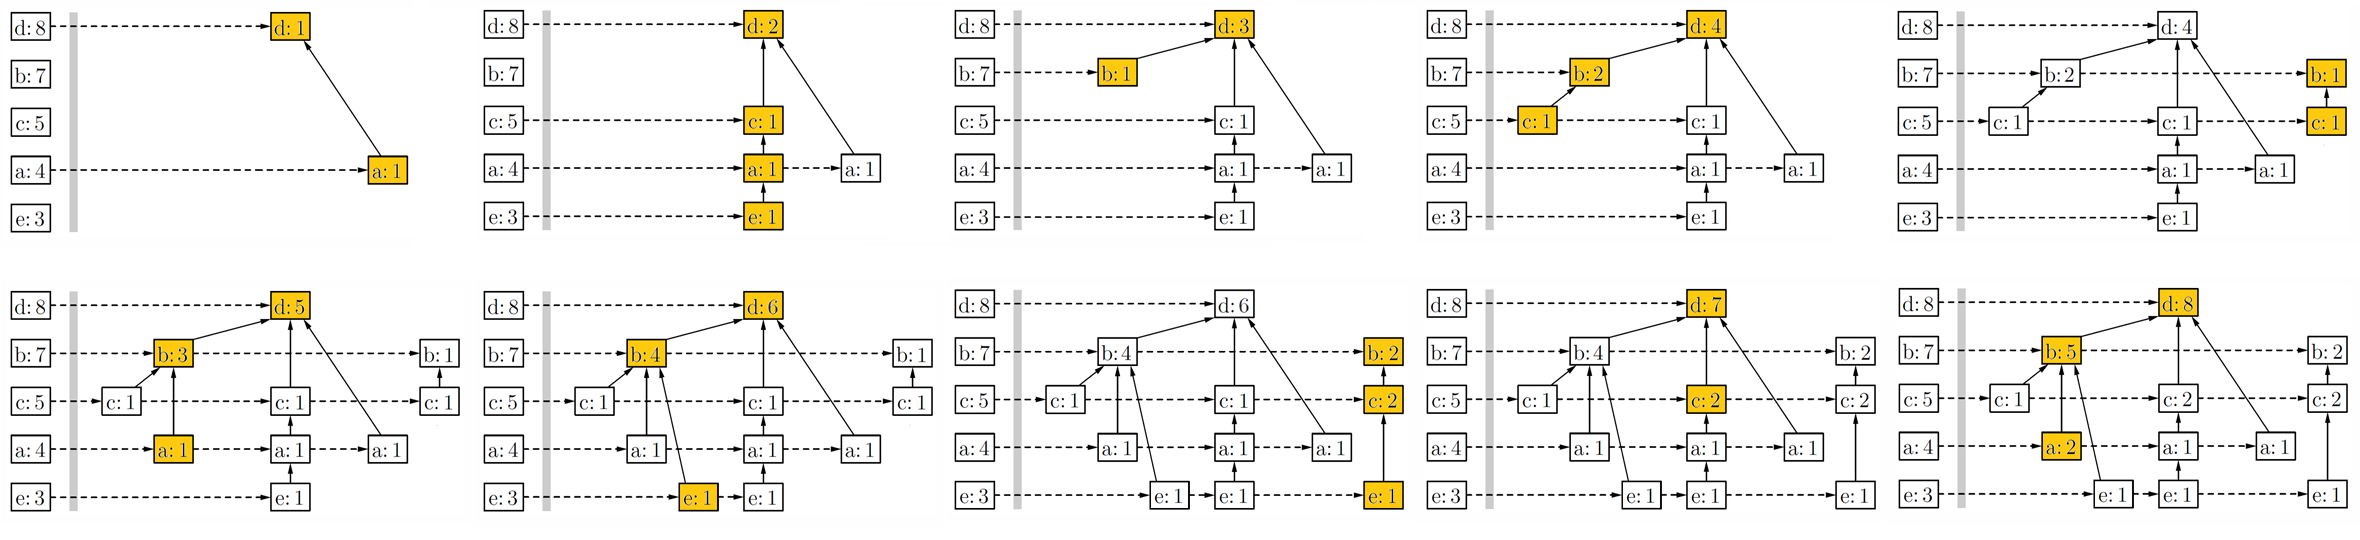
\includegraphics[width=1\linewidth]{chapters/rules/images/fp-tree-stages-example.png}
    \caption{Иллюстрация этапов построения FP-дерева}
    \label{fig:enter-label}
\end{figure}

\textbf{Введём обозначения:}

\begin{itemize}
    \item $V(T, f) = {v \in T: f_v = f}$ - все вершины, соответствующие признаку $f$. Соответственно, у них равные глубины.
    \item $C(T, f) = \displaystyle\sum_{v \in V(T, f)} c_v$ - Сумма счетчиков вершин, соответствующих признаку $f$. Несложно понять, что эта сумма равна числу объектов $x_i \in U$, для которых $f(x_i) = 1$. Другими словами $C(T, f) = l\nu(f)$
\end{itemize}


\subsection{Построение условного FP-дерева}

Прежде чем приступить к второму этапу алгоритма, разберёмся в одной важной для него процедуре. 
\newline\newline
\textbf{Определение.} Пусть FP-дерево $T$ построено по подвыборке $U$. Условное FP-дерево $T' = T|\varphi$ - это FP-дерево, порождаемое подвыборкой $\{x_i \in U| \varphi(x_i) = 1 \}$ из которого удалены все вершины признака $f$ и ниже.
\newline\newline
Рассмотрим алгоритм построения $T|f$ по $T$, где $f$ - признак из $\mathcal{F}$:
\begin{enumerate}
    \item Оставим в дереве только те вершины, которые принадлежат путям, идущим от вершин признака $f$ до корня. 
    \item Обновим счетчики $c_i$: для вершин признака $f$ ничего не меняем, а для остальных рекурсивно снизу вверх обновляем по формуле $c_u = \displaystyle\sum_{w \in S_u} c_w$
    \item Удаляем вершины признака $f$ из $T'$.
\end{enumerate}

Корректность следует из построения.

\subsection{Построение списка ассоциативных правил}

Для начала поймем, как эффективно находить $\nu(\varphi)$ используя FP-дерево. Для этого мы можем просто найти $f =argmin_{f \in \varphi} (\nu(f))$ и просуммировать $c_v$ для всех вершин $v$ признака $f$, таких что $\varphi \subset [f_{v_0}, f_{v}]$, где $[f_{v_0}, f_{v}]$ - набор признаков $f_{v_i}$ вершин из пути от корня до $v$.
\newline\newline
Рассмотрим функцию FP-find$(T,\varphi,R)$, которая находит по FP-дереву $T$, все частные наборы, содержащие только частный набор $\varphi$, и признаки, которые в FP-дереве стотят выше всех признаков из $\varphi$, и добавляет их в список $R$. Она играет ключевую роль в работе данного алгоритма. Вот как её можно реализовать:
\newline\newline
\textbf{Псевдокод:}

\noindent\hrulefill % Горизонтальная линия
\begin{enumerate}
    \item \textbf{ПРОЦЕДУРА} FP-find$(T,\varphi,R)$;
    \newline
    \quad \textit{Вход:} $T$ — FP-дерево, частный набор $\varphi$, список наборов $R$.
    \newline
    \quad \textit{Выход:} Добавить все частные наборы, содержащие $\varphi$ в $R$.
    \item \quad для всех $f \in \mathcal{F} : V(T,f) \neq \emptyset$ по уровням снизу вверх:
    \item \quad \quad если $C(T,f) \geq l\delta$ то:
    \item \quad \quad \quad набор $\varphi \cup \{f\}$ - частый, добавляем его в $R$;
    \item \quad \quad \quad $T':=T|f$ - условное FP-дерево;
    \item \quad \quad \quad FP-find$(T',\varphi \cup \{f\},R)$; - рекурсивно найти все частые наборы, содержащие $\varphi \cup \{f\}$
\end{enumerate}
\noindent\hrulefill % Горизонтальная линия
\newline\newline
Для получения списка всех частых наборов, мы можем просто запустить FP-find$(T,\emptyset,\emptyset)$. Алгоритм просмотрит все наборы в обратном лексикографическом порядке. Для выделения ассоциативных правил теперь можем запустить функцию AssocRules из алгоритма APriory.

\subsection{Задачи для практики}
\textbf{Задача 1.} Как используя FP-дерево, построенное по выборке $U$ найти а) самый частый набор, б) самый редкий набор?
\newline\newline
\textbf{Решение.} 
\newline
а) По свойству антимонотонности, один из наборов размера 1 будет самым часто встречаемым. Так как признаки в FP-дереве уже отсортированы по частоте, самым частым будет самый верхний. Сложность алгоритма получается равной $O(1)$.
\newline
б) Подмножество каждого пути из корня в FP-дереве соответствует какому-то набору. Также каждый набор, соответствующий строке в базе, соответствует какому-то пути в дереве. По свойству антимонотонности, одним из наборов, соответствующих путям из корня до листьев, должен быть самым редким. Количество упоминаний одного из таких наборов - это значение счетчика $c_v$ в соответствующем листе. То есть наша задача сводится к поиску листа с минимальным значением этого счетчика. Это можно сделать, пройдя обходом в глубину по всему дереву, за $O(2^n)$, где $n$ - глубина дерева в худшем случае.
\newline\newline
\textbf{Задача 2.} Как по уже построенному FP-дереву для выборки $U$ и фиксированных параметров поддержки $\delta$ и значимости $\chi$, найти все ассоциативные правила, удовлетворяющие $\delta, \chi$ вида $a \to b$, где $a,b \in \mathcal{F}$ за $O(n2^n)$ в худшем случае?
\newline\newline
\textbf{Решение.} 
\newline
Заметим, что всего таких правил порядка $n^2$, где $n$ - число признаков. То есть для того, чтобы дать ответ, нам достаточно найти $\nu(f), \nu(f \cup g)$ для всех признаков $f,g$ из дерева. Первые величины уже известны, так как были вычислены на первом этапе построения FP-дерева. Для нахождения всех $\nu(f \cup g)$, достаточно создать двумерный массив $C$, такой что $C_{fg}$ равно числу $x \in U: (f \wedge g)(x_i) = 1$. Для его заполнения мы можем пройти обходом в глубину по дереву, и находясь в вершине $v$, прибавлять $c_v$ к $C_{f_vf_u} = C_{f_uf_v}$ для всех $u \in [v_0, v]$, где $ [v_0, v]$ - путь от корня до $v$. Этот обход потребует порядка $O(n2^n)$ действий. То есть суммарно у нас уйдет $O(n2^n + n^2) = O(n2^n)$ действий.
\newline\newline
\textbf{Задача 3.}
Оцените время работы алгоритма FP-Growth для нахождения ассоциативных правил, удовлетворяющих поддержке $\delta$ и значимости $\chi$ в худшем случае.
\newline\newline
\textbf{Решение.} 
\newline
Если с временем построения FP-дерева все понятно - оно совпадает с временем построения бора по массиву строк и равно $O(nl)$. То асимптотика генерации всех частых наборов и выделение ассоциативных правил значительно труднее для вычисления. Построение условного FP-дерева $T|f$ по самому нижнему признаку $f$ выполняется одним обходом в глубину - асимптотически $O(2^n)$. Пусть FP-find$(T,\emptyset,\emptyset)$ выполняется за время $k(n)$, тогда $k(n) = O\left(\sum_{i = 0}^{n-1} (2^i + k(i))\right)$, где $2^i$ действий уходит на построение условного дерева по каждому из признаков. Сделаем замену $t(n):=2^n+k(n)$, тогда $t(n) - 2^n = O\left(\sum_{i = 0}^{n-1}t(i)\right)$, заметим, что для $t(n) = n2^n$ верно: $n2^n = O\left(\sum_{i = 0}^{n-1} i2^i\right) = O((n-2)2^n)$. Значит $k(n) = O(n2^n)$. Теперь найдем время выделения ассоциативных правил. Операция нахождения $\nu(\varphi)$ по данному $\varphi$ может быть оптимизирована с использованием дерева поиска для хранения множества $\varphi$, что даст суммарное время работы $O(nlogn + 2^d\cdot \log(n)) = O((2^d + n)\cdot \log(n))$, где $d$ - глубина самого нижнего признака из $\varphi$. Для выделение ассоциативных правил из набора $\varphi$ длинны $k$, время упирается в скорость вычисления $\nu(\varphi')$ для проверки $\nu(y' | \varphi') \geq \chi$, поэтому оно будет не хуже, чем $O(2^k \cdot (2^d + n)\cdot \log(n)))$, и не лучше $O(2^{k-1} \cdot (2^d + n)\cdot \log(n)))$ - так как есть $2^{k-1}$ набор содержащий признак глубины $d$, поддержку которого надо вычислить. Наконец выделение всех ассоциативных правил для всех частых наборов в худшем случае будет порядка 
$$O\left(\sum_{d = 1}^{n} \sum_{k = 1}^{n-d} \mathrm{C}_{n-d}^{k} \cdot 2^{k-d}\cdot \log(n) \right) =
O\left(\sum_{d = 1}^{n} \frac{3^{n-d}}{2^d} \cdot\log(n) \right) =O(3^n \log(n))  $$
Что и будет решающим слагаемым в асимптотике работы всего алгоритма.


\section{Алгоритм APriory}

\subsection{Свойство антимонотонности}
Алгоритм \textbf{APriory} основывается на свойстве \textbf{антимонотонности} функции \( \varphi(x)= \bigwedge_{f \in \varphi} f(x)\):

Для любых \( \psi, \varphi \subset \mathcal{F} \), из \( \varphi \subset \psi \) следует \( \nu(\varphi) \geq \nu(\psi) \).

\textbf{Следствия:}

\begin{enumerate}
    \item Если \( \psi \) частый, то все его подмножества \( \varphi \subset \psi \) частые.
    \item Если \( \varphi \) не частый, то все наборы \( \psi \supset \varphi \) также не частые.
    \item \( \nu(\varphi \cup \psi) \leq \nu(\varphi) \) для любых \( \varphi, \psi \).
\end{enumerate}

Основываясь на этих свойствах, мы можем построить итеративный алгоритм нахождения ассоциативных правил (\textbf{APriory}). Алгоритм состоит из двух этапов:

\begin{enumerate}
    \item Поиск частых наборов 
    \item Выделение ассоциативных правил
\end{enumerate}

Вторая часть алгоритма считается полностью \textit{решенной}, так как существует простая и эффективная процедура, реализующая её. Первая же часть представляет наибольший интерес, так как требует многократное обращение к базе данных, поэтому стоит важный вопрос оптимизации этого этапа.

\subsection{Поиск частых наборов}

\textbf{Идея алгоритма:} на \( j\) этапе храним все \textit{частые наборы} мощности \(j\): \(G_j\). Тогда при переходе от \(G_j\) к \(G_{j+1}\) пытаемся увеличить каждое из множеств \(\varphi \in G_j\), чтобы оно по-прежнему оставалось \textit{частым набором}.
\newline\newline
\textbf{Псевдокод:}
\newline
\textit{Вход:} \( X^\ell \) — обучающая выборка; минимальная поддержка \( \delta \); минимальная значимость \( \chi \).
\newline
\textit{Выход:} \( R = \{(\varphi, \psi)\} \) — список ассоциативных правил.

\noindent\hrulefill % Горизонтальная линия
\begin{enumerate}
    \item Множество \textbf{всех частых} исходных признаков: \newline
    \(G_1 := \{ f \in \mathcal{F} \mid \nu(f) \geq \delta \};\)
    
    \item \textbf{Для всех} \( j = 2, \ldots, n \):
     \item \quad Множество \textbf{всех частых} наборов мощности \( j \): 
     \[
     G_j := \{ \varphi \cup \{f\} \mid \varphi \in G_{j-1}, \, f \in G_1, \, \nu(\varphi \cup \{f\}) \geq \delta \};
    \] 
        \item \quad \textbf{Если} \( G_j = \emptyset \), то:
            \item \quad  \quad\textbf{выход} из цикла по \( j \);
    \item \( R := \emptyset \);
    \item \textbf{Для всех} \( \psi \in G_j, \, j = 2, \ldots, n \):
    \item \quad \texttt{AssocRules}( \( R, \psi, \emptyset \) );
\end{enumerate}
\noindent\hrulefill % Горизонтальная линия
\newline

Заметим, что за лаконичной математической формулой \(\nu(\varphi \cup \{f\}) \geq \delta \) на самом деле скрывается просмотр базы данных, что делает эту проверку очень тяжелой. 

\subsection{Выделение ассоциативных правил.}
\textbf{Идея алгоритма:} \textit{отщипываем} по одному признаку из \(\varphi\), проверяем ассоциативность получившегося правила.
\newline\newline
\textbf{Псевдокод:}
\newline
\textit{Вход:} $R$ — список ассоциативных правил; \\
\textit{Выход:} $(\varphi, y)$ — ассоциативное правило;

\noindent\hrulefill % Горизонтальная линия
\begin{enumerate}
    \item \textbf{ПРОЦЕДУРА} AssocRules $(R, \varphi, y)$;
    \item \quad \textbf{для всех} $f \in \varphi$
    \item \quad \quad $\varphi' := \varphi \setminus \{f\}$; \quad $y' := y \cup \{f\}$;
    \item \quad \quad \textbf{если} $\nu(y' | \varphi') \geq \chi$ \textbf{то}
    \item \quad \quad \quad добавить ассоциативное правило $(\varphi', y')$ в список $R$;
    \item \quad \quad \textbf{если} $|\varphi'| > 1$ \textbf{то}
    \item \quad \quad \quad AssocRules $(\varphi', y')$;
\end{enumerate}
\noindent\hrulefill % Горизонтальная линия
\newline
\subsection{Задачи для практики}

\subsubsection{Задача 1: Простота алгоритма APriory:} Чтобы лучше прочувствовать алгоритм APriory (а также убедиться в его простоте) проделайте его руками для следующей таблицы транзакций (числа - номера транзакции, буквы - признаки), а именно найдите все частые наборы признаков (\(G_1, G_2, \ldots)\)) при \( \text{minsup}=0.3 \).
\begin{table}[ht!]
\centering
\caption{Таблица транзакций}
\begin{tabular}{ccccccc}
\toprule
\textbf{Транзакция} & \textbf{A} & \textbf{B} & \textbf{C} & \textbf{D} & \textbf{E} & \textbf{F} \\
\midrule
1  & 1 & 1 & 1 & 0 & 0 & 0 \\
2  & 1 & 0 & 1 & 1 & 0 & 0 \\
3  & 0 & 1 & 1 & 1 & 1 & 0 \\
4  & 1 & 1 & 0 & 1 & 0 & 1 \\
5  & 1 & 0 & 1 & 1 & 1 & 0 \\
6  & 0 & 1 & 1 & 0 & 0 & 0 \\
7  & 1 & 1 & 1 & 0 & 1 & 0 \\
8  & 1 & 0 & 0 & 1 & 1 & 1 \\
9  & 0 & 1 & 1 & 1 & 0 & 0 \\
10 & 1 & 1 & 1 & 0 & 1 & 0 \\
\bottomrule
\end{tabular}
\end{table}
\newline
\textit{Решение:}

\textbf{Шаг 1: Частые одноэлементные наборы (\( G_1 \))}

Считаем поддержку для каждого элемента:
\[
\begin{aligned}
&\{A\}: 7, \quad \{B\}: 6, \quad \{C\}: 8, \quad \{D\}: 6, \quad \{E\}: 5, \quad \{F\}: 2.
\end{aligned}
\]

Частые одноэлементные наборы (\( support \geq 3 \)):

\[
G_1 = \{\{A\}, \{B\}, \{C\}, \{D\}, \{E\}\}.
\]

\textbf{Шаг 2: Частые пары (\( G_2 \))}

Формируем все возможные пары элементов (\( \varphi_2 \)) и считаем их поддержку:

\[
\begin{aligned}
&\{A, B\}: 4, \quad \{A, C\}: 4, \quad \{A, D\}: 4, \quad \{A, E\}: 4, \\
&\{B, C\}: 6, \quad \{B, D\}: 3, \quad \{B, E\}: 3, \\
&\{C, D\}: 4, \quad \{C, E\}: 4, \quad \{D, E\}: 3.
\end{aligned}
\]

Частые пары (\( support \geq 3 \)):

\[
G_2 = \{\{A, B\}, \{A, C\}, \{A, D\}, \{A, E\}, \{B, C\}, \{B, D\}, \{B, E\}, \{C, D\}, \{C, E\}, \{D, E\}\}.
\]

\textbf{Шаг 3: Частые тройки (\( G_3 \))}

Формируем тройки (\( \varphi_3 \)) и считаем их поддержку:

\[
\begin{aligned}
&\{A, B, C\}: 3, \quad \{A, B, D\}: 1, \quad \{A, B, E\}: 1, \\
&\{A, C, D\}: 2, \quad \{A, C, E\}: 3, \quad \{A, D, E\}: 1, \\
&\{B, C, D\}: 2, \quad \{B, C, E\}: 3, \quad \{B, D, E\}: 1, \\
&\{C, D, E\}: 1.
\end{aligned}
\]

Частые тройки (\( support \geq 3 \)):

\[
G_3 = \{\{A, B, C\}, \{A, C, E\}, \{B, C, E\}\}.
\]

\textbf{Шаг 4: Частые четверки (\( G_4 \))}

Формируем четверки (\( \varphi_4 \)):

\[
\{A, B, C, E\}: 1.
\]

Поддержка меньше минимальной (\( support < 3 \)), поэтому завершаем алгоритм.

\subsubsection{Задача 2: Сложность алгоритма APriory:} К.В. Воронцов так отзывался об алгоритме APriory: "Простой, классический, везде описанный, но пользоваться им не надо". Мы уже упоминали о неэффективности этого алгоритма, теперь убедитесь в этом сами: посчитайте временную асимптотику и асимптотику используемой памяти (обозначим \(|D|\) - количество признаков)


\textit{Решение:} Если размер максимального по включению частого множества \(|S|\), то мы переберем также все его подмножества, то есть пройдет \(\mathcal{O}(2^{|S|})\) итераций. Итого асимптотика \(\mathcal{O}(2^{|D|})\)

Пусть снова \(S\) - максимальное частое множество. Значит все его подмножества - также частые множества, значит они также будут сохранены, значит памяти будет занято \(\mathcal{O}(2^{|S|})\). Итоговая асимптотика памяти \(\mathcal{O}(2^{|D|})\).

Основная проблема алгоритма - мы наивно ищем частые наборы. Следующий алгоритм \textit{FP-Growth} признан решить эту проблему, используя эффективные структуры данных для быстрого поиска.

\subsubsection{Задача 3: Недостатки алгоритма APriory на практике:} В прошлой задаче мы убедились в неэффективности алгоритма с точки зрения его временной сложности. Подумайте теперь о недостатках алгоритма при его использовании на практике (не считая временной сложности). Для ответа вспомните примеры использования ассоциативных правил в жизни.

\textit{Решение:} Вспомнил классический пример применения поиска ассоциативных правил — анализ рыночной корзины. При непосредственном использовании алгоритма, где товары рассматриваются как признаки, а чеки — как объекты, возникает важная проблема: нам необходимо не просто анализировать отдельные товары, а учитывать сгруппированные категории. Например, нас интересует не просто покупка конкретных видов хлеба, а сам факт приобретения хлебобулочных изделий (или, например, приобретения черного хлеба). Таким образом, нужно учитывать иерархию признаков.

Другая проблема - мы никак не учитываем информацию о самих клиентах (например, семейное положение, возраст\(\ldots\)). На практике при построении ассоциативных правил эта информация сильно влияет на правила, поэтому их нельзя игнорировать.

\section{Алгоритм RARM.}

\subsection{Информация об алгоритме}

Алгоритм Apriori зачастую работает достаточно медленно, поэтому придуман алгоритм, который на практике работает в 10-100 раз быстрее, чем алгоритм Apriori

\begin{enumerate}
    \item \textbf{Идея ускорения:}
    \begin{itemize}
        \item Алгоритм RARM направлен на преодоление ограничений по скорости, существующих в классических методах ассоциативного анализа, таких как Apriori.
        \item Используется специальная структура данных, называемая \textbf{Support-Ordered Trie itemset (SOTrieIT)}, для хранения предварительно обработанных транзакционных данных.
    \end{itemize}

    \item \textbf{Особенности SOTrieIT:}
    \begin{itemize}
        \item Эта структура позволяет RARM быстро генерировать частые наборы из одного элемента (\textit{1-itemsets}) и двух элементов (\textit{2-itemsets}).
        \item Алгоритм не требует повторного сканирования базы данных и не создает кандидатов для \textit{2-itemsets}, что обычно является узким местом алгоритма Apriori.
    \end{itemize}

    \item \textbf{Превосходство над Apriori:}
    \begin{itemize}
        \item Главным узким местом Apriori является генерация кандидатов для \textit{2-itemsets}. RARM устраняет эту проблему, что значительно увеличивает его скорость.
        \item Как и было сказано, в сравнении с Apriori RARM демонстрирует значительное ускорение --- до \textbf{100 раз быстрее}.
    \end{itemize}

    \item \textbf{Практическая значимость:}
    \begin{itemize}
        \item Алгоритм RARM превосходит не только Apriori, но и другие современные алгоритмы ассоциативного анализа по скорости.
    \end{itemize}
\end{enumerate}

Таким образом, RARM предлагает инновационный подход для ассоциативного анализа, устраняя основные узкие места традиционных методов за счёт эффективного представления данных и оптимизированных процессов обработки.

\subsection{Оценка времени алгоритма}

Для сравнения временной сложности алгоритмов RARM и Apriori, мы сосредоточимся только на процессе сканирования базы данных для получения поддержек наборов элементов. Этого достаточно, чтобы увидеть значительное улучшение RARM по сравнению с Apriori.

Для каждого прохода алгоритма Apriori необходимо сканировать всю базу данных, независимо от желаемого порога поддержки. Пусть размер базы данных равен \(a\), а средний размер каждой транзакции — \(b\). Тогда Apriori требует \(O(ab)\) единиц времени для сканирования базы данных на каждом проходе.

Для первых двух проходов алгоритма RARM необходимо сканировать структуру SOTrieIT Y. SOTrieIT(при желании можно изучить эту структуру подробнее), \texttt{Y} имеет \(R \times C\) узлов, и поскольку каждый узел имеет одну ссылку от своего родителя, в худшем случае потребуется не более \(2 \times R \times C\) единиц времени для обхода всей структуры, где \(N < a\). Кроме того, время, необходимое для сканирования, также зависит от желаемого порога поддержки, что дополнительно уменьшает количество обходов. Таким образом, среднее общее количество времени для сканирования будет гораздо меньше, чем \(O(ab)\).

\subsection{Задачи}

\subsubsection{Задача 1: Сравнение по времени с FP-деревом} Мы знаем про существование FP-дерева. Что из них эффективнее на практике по времени и насколько?

\textbf{Решение.} 

\begin{itemize}
    \item \textbf{RARM} обычно выигрывает по скорости, когда требуется быстрое извлечение частых 1- и 2-itemsets, особенно для больших данных, где минимизация сканирований и генерации кандидатов важна.
    \item \textbf{FP-дерево} имеет отличную производительность, особенно когда нужно работать с более глубокими паттернами, но может страдать от роста сложности при большом количестве элементов и комбинаций.
\end{itemize}

В целом, \textbf{RARM} может быть предпочтительным, если основное внимание уделяется скорости на начальных этапах, тогда как \textbf{FP-tree} подходит для более универсальных решений с различной глубиной паттернов.


\subsubsection{Задача 2: Сравнение по памяти с FP-деревом} Теперь мы хотим узнать, что больше подойдет по памяти - FP-дерево или RARM?

\textbf{Решение.} 

\begin{itemize}
    \item \textbf{RARM} имеет преимущество в использовании памяти на начальных этапах, когда анализируются только 1- и 2-itemsets. Он эффективно управляет памятью при больших объемах данных, особенно на первых этапах обработки.
    \item \textbf{FP-tree} использует сжатие транзакций и может быть более эффективным в плане памяти для баз данных с высокой поддержкой паттернов, но может страдать от увеличения объема памяти при большом количестве уникальных элементов.
\end{itemize}

\subsubsection{Задача 3: Сравнение по скорости} Насколько эффективнее RARM по времени относительно Apriori?

\textbf{Решение.} 

Практические данные действительно показывают, что Apriori всегда работает медленнее, чем RARM, однако при изучении k-itemsets, где k > 3 алгоритм RARM показывает себя не значительно лучше, чем Apriori так как RARM использует Apriori в их изучении. Однако на всех других данных, алгоритм RARM показывает улучшение по времени вплоть до 120 раз относительно Apriori



\section{Задача автоматического выделения терминов: алгоритм TopMine, UDPipe, модель PLSA.}

Цель для такой задачи является выделение составных терминов в текстовых коллекциях. Термин - фраза (n-грамма) со следующим набором свойств:

\begin{itemize}
	\item Высокая частотность - много раз встречается в коллекции.
	\item Контактная сочетаемость слов - состоит из слов, неслучайно часто встречающихся вместе.
	\item Полнота - является максимальной по включению цепочкой слов.
	\item Синтактическая свяхность - является грамматически корректным словосочетанием.
	\item Тематичность - часто встречается в узком подмножестве тем.
\end{itemize}

Для проверки каждой из свойств используются 

\begin{itemize}
	\item Статистический анализ: для проверки первых трёх свойств терминов. Он позваляет находить высокочастотные токены, выделять слова, неслучайно стоящие рядом и штрафовать неполные последовательности слов, входящие как подмножество в другую высокочастотную последовательность неслучайно стоящих слов.
	\item Синтаксический анализ: для проверки синтактической связности. Данный анализ позволяет выделять синтактически связанные словосочетания в предложениях.
	\item Тематическая модель: для проверки тематичности. Она позволяет сопоставить каждому токену распределение тем.
\end{itemize}

Для каждого анализа мы будем использовать модели TopMine, UDPipe и PLSA для семантического, синтаксического анализа и тематической модели соответственно. Рассмотрим в подробности каждую модель

\subsection*{Статистический анализ: TopMine}

Этот алгоритм итеративно сливает слова и фразы в предложении, рассчитывая для каждого слияния оценку значимости \textit{SignificanceScore} и останавливается, когда для всех возможных слияний значимость меньше заданного порога. 

В начале мы должны найти все частые k-грамм и алгоритм быстрого поиска приведён на рисунке 1.
\begin{figure}
    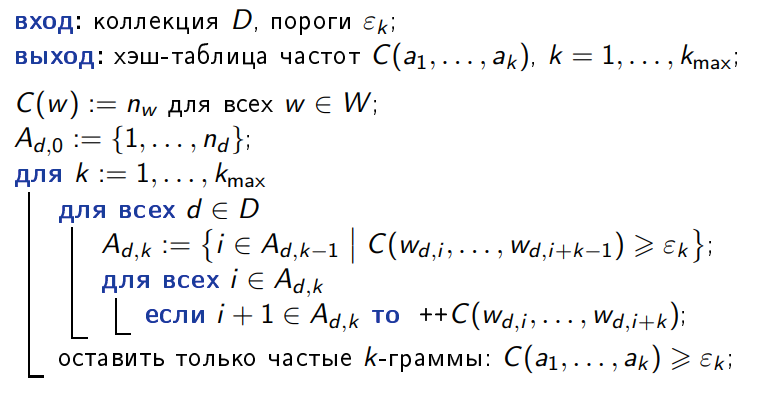
\includegraphics[scale = 0.5]{chapters/rules/images/ml1.png}
    \caption{Алгоритм быстрого поиска}
\end{figure}
где $C(a_{1},...,a_{k})$ - хэш-таблица частот k-грамм, $a_{i} \in W$, $C(w) = n_{w}$ для всех униграмм $w \in W: n_{w} \geq \varepsilon_{1}$, где $W$ - множество слов или фраз.
$\varepsilon_{1}$ - пороговое значение частоты частых k-грамм
$A_{d,k}$ - множество позиций i в документе d, с которых начинаются все частые k-граммы
$C(w_{d,i},...,w_{d,i+k-1}) \geq \varepsilon_{k}$
Свойство антимонотонности: $C(a_{1},...,a_{k}) \geq C(a_{1},...,a{k+1})$

Затем должны провести итеративное слияние фраз с понижением значимости до $\alpha$.
$SignificanceScore = \frac{p_{uv}-p_{u}p_{v}}{\sqrt{p_{uv}}}$
где $p_{u}$ - оценка вероятности встретить фразу \textit{u}, $p_{uv}$ = оценка вероятности встретить фразу \textit{uv}.

В начале у нас есть кортеж исходных фраз и первой итерацией считается \textit{SignificanceScore} для всех соседних пар фраз. И затем из кортежа удаляются все все пары с \textit{SignificanceScore} больше $\alpha$. Оставшиеся элементы в кортеже и являются термами. На рисунке 2 приведен пример работы алгоритма TopMine.
\begin{figure}
    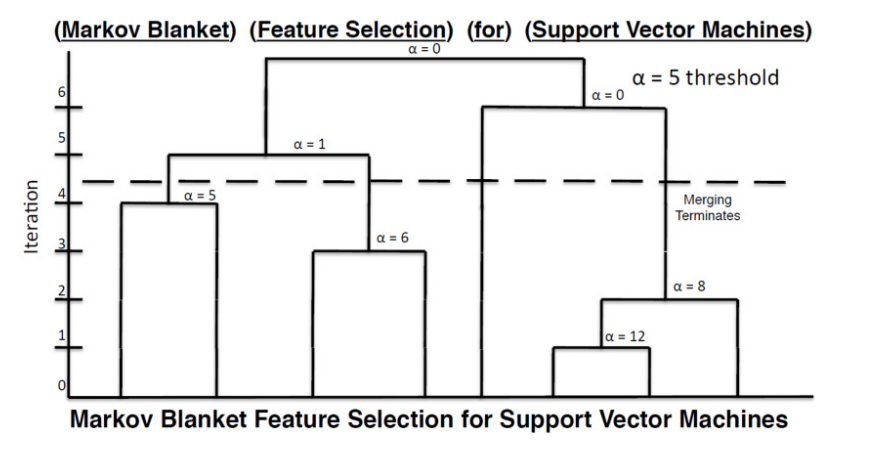
\includegraphics[scale = 0.5]{chapters/rules/images/ml2.png}
    \caption{Пример работы алгоритма TopMine}
\end{figure}
\subsection*{Синтаксический анализ: UDPipe}

UDPipe - предобученная модель, которая может распозновать синтаксические связи в предложениях и разметка частей речи слов в предложениях. На вход подаётся список предложений, и для каждого слова в предложениях вычисляется:

\begin{itemize}
	\item Часть речи слова.
	\item Член предложения.
	\item ID родительского слова.
\end{itemize}

Модель для каждого предложения создаёт синтаксическое дерево, и при помощи неё проверяет словосочетании-кандидаты. Для них подсчитывается оценка его синтаксической связанности по формуле $SyntaxScore(W) = max SyntaxDistance(w_{i}, w_{j})$, где \textit{W} - N-грамма, $1 \leq i \leq N$, $1 \leq j \leq N$ и $i \neq j$.Таким образом, если одно из слов в словосочетании-кандидате синтактически не связанно с остальным, \textit{SyntaxScore} это выявит.

\subsection*{Тематический анализ: PLSA}

У нас есть коллекция текстовых документов $D$ и словарь токенов $W$, из которых состоят документы. Каждый документ $d \in D$ представляет собой последовательностью входящих в него токенов из словаря $W$. Если предположить, что местоположение токенов в документе не влияет на определение тематики документа, то документ это подмножество $d \subset W$, в котором каждому токену $w \in d$ поставлено в соответствие число $n_{dw}$ вхождений в документ $d$.

Модель описывает вероятности появления токенов $w$ в документов $d$ при предположении условной независимости:
$$p(w|d) = \sum_{t \in T} p(w|t)p(t|d) = \sum_{t \in T} \phi_{wt} \theta_{td}$$
где $\phi_{wt} = p(w|t), \theta_{td} = p(t|d)$ являются обучаемыми параметрами модели. Для обучения параметров модели, представленные в виде матрицы $\Phi = (\phi_{wt})_{WxT}$ и $\Theta = (\theta_{td})_{TxD}$ по коллекции документов $D$ максимизируется логарифм правдоподобия
$$L(\Phi, \Theta) = \sum_{d \in D} \sum_{w \in d} n_{dw} ln \sum_{t \in T} \phi_{wt} \theta_{td} \rightarrow \max_{\Phi, \Theta}$$

при ограничениях неотрицательности и нормировки
$$\sum_{w \in W} \phi_{wt} = 1, \phi_wt \geq 0, \sum_{t \in T} \theta_{td} = 1, \theta_{td} \geq 0$$

На основе полученных параметров $\Phi$ и $\Theta$ для каждого словосочетания-кандидата считается распределение тем $p(t|w) = \phi_{wt} \frac{p(t)}{p(w)}$. Отбор происходит распределением тематик $p(t|w)$ имеет высокую вероятность только для некоторых тем из малого подмножества всех тем T. Это можно оценить через отдаленность $p = p(t|w)$ от равномерного $p_{unif} = 1/T$, где $T$-мощьность множества $T$. Расстояние между двумя распределениями считается несколькими способами:

\begin{itemize}
	\item Дивергенция Кульбака-Лейблера
	$$KL(pp_{unif}) = \sum_{t \in T} \frac{1}{|T|} ln \frac{\frac{1}{|T|}}{p(t|w)}$$
	\item Дивергенция Йесена-Шеннона
	$$JS(pp_{unif}) = \frac{1}{2}KL(p_{unif}p_{1}) + \frac{1}{2}KL(pp_{1})$$
	$$p_{1}(t|w) = \frac{1}{2}(p(t|w) + \frac{1}{|T|})$$
	\item Сумма степенных функций, $\gamma > 1$
	$$Deg(p) = \sum_{t \in T} p(t|w)^{\gamma}$$
\end{itemize}

Чем больше значение данных метрик для $w$, тем тематичнее данная N-грамма.

\subsection*{Задачи}

\textbf{Задача 1.} Нам дана фраза \textit{a} \textit{b}, было оценено вероятность встречи фраз $p_{a} = 0,1$, $p_{b} = 0,2$, $p_{ab} = 0,05$. Пороговая значимость $\alpha = 1$. Является ли фраза \textit{ab} термином?

\textbf{Ответ:} Нет.

\textbf{Решение.} 
$$\frac{p_{ab}-p_{a}p_{b}}{\sqrt{p_{ab}}} \approx 0,01 < \alpha$$

 \textbf{Задача 2.} Дано синтактическое дерево (рис. 3) для предложения "An inventory of syntactic functions is taken to be primitive". Найдите \textit{SyntaxScore} для фразы "syntactic functions is".
 
\begin{figure}
    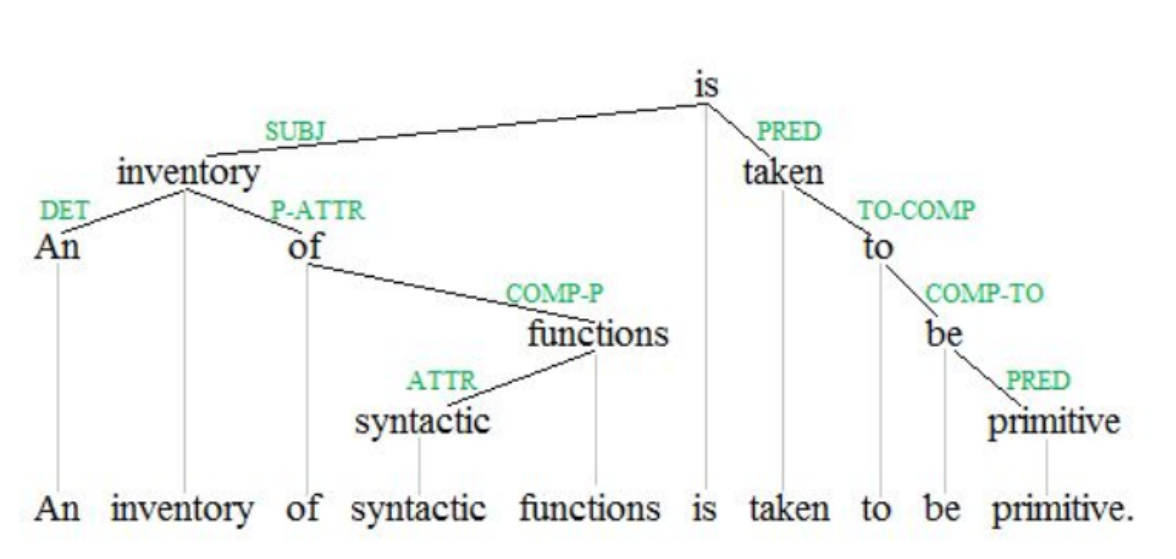
\includegraphics[scale = 0.4]{chapters/rules/images/ml3.png}
    \caption{Задача 2}
\end{figure}

\textbf{Ответ:} 4.

\textbf{Задача 3.} Привести аналитическое решение максимизации задачи

$$L(\Phi, \Theta) = \sum_{d \in D} \sum_{w \in d} n_{dw} ln \sum_{t \in T} \phi_{wt} \theta_{td} \rightarrow \max_{\Phi, \Theta}$$

и выразить элементы матрицы $\Phi$ и $\Theta$ через $n_{dw}$ и $p(t|d,w)$.

\textbf{Решение.}

Запишем лангранжиан задачи, учитывая ограничение нормировки:

$$L(\Phi, \Theta) = \sum_{d \in D} \sum_{w \in d} n_{dw} ln \sum_{t \in T} \phi_{wt} \theta_{td} - \sum_{t \in T} \lambda_{t} (\sum_{w \in d} \phi_{wt} - 1) - \sum_{d \in D} \mu_{d} (\sum_{t \in T} \theta_{td} - 1)$$

Продифференцируем лангранжиан по $\phi_{wt}$ и приравняем к нулю производную, получим:

$$\lambda_{t} = \sum_{d \in D} n_{ds} \frac{\theta_{td}}{p(w|d)}$$

Домножив обе части на $\phi_{wt}$, получим:

$$\lambda_{t} \phi_{wt} = \sum_{d \in D} n_{ds} \frac{\phi_{wt} \theta_{td}}{p(w|d)}$$

По формуле Байеса:

$$p(t|d,w) = \frac{p(w|t) p(t|d)}{p(w|d)} = \frac{\phi_{wt} \theta_{td}}{p(w|d)}$$

Сделав замену  получим:

$$\lambda_{t} \phi_{wt} = \sum_{d \in D} n_{ds} p(t|d,w)$$

Просуммируем по $w \in W$ и получим:

$$\lambda_{t} \sum_{w \in W} \phi_{wt} = \sum_{w \in W} \sum_{d \in D} n_{ds} p(t|d,w)$$

В соответствии с условием нормировки $\sum_{w \in W} \phi_{wt} = 1$:

$$\lambda_{t} = \sum_{w \in W} \sum_{d \in D} n_{ds} p(t|d,w)$$

Выразив из $\lambda_t \phi_{wt} = \sum_{d \in D} n_{dw} p(t|d,w)$ $\phi_{wt}$ и подставив $\lambda_{t}$ получаем:

$$\phi_{wt} = \frac{\sum_{d \in D} n_{dw} p(t|d,w)}{\sum_{w_{1} \in W} \sum_{d \in D} n_{dw_{1}} p(t|d,w_{1})}$$

Для $\theta_td$ поступаем аналогично. После приравнивания производной по $\theta_{td}$ к $0$, домнажения на $\theta_{td}$, суммирования по всем $t \in T$ находим $\mu_{d}$:

$$\mu_{d} = \sum_{t \in T} \sum_{w \in d} n_{dw} p(t|d,w)$$

Выразим $\theta_{td}$:

$$\theta_{td} = \frac{\sum_{w \in d} n_{dw} p(t|d,w)}{\sum_{w \in d} n_{dw} \sum_{t_{1} \in T} p(t_{1}|d,w)}$$


\section{\textbf{\textit{ECLAT (Equivalence Class Transformation) алгоритм}}}
\textbf{\textit{Prerequisites:}} Задача поиска ассоциативных правил: определения/прикладные задачи/связь с логическими закономерностями, \textit{Apriori} алгоритм.\newline\newline
\textit{ECLAT} — это эффективный алгоритм для поиска частых наборов элементов с использованием вертикального представления данных. Его основная идея заключается в том, чтобы представлять данные в виде списка идентификаторов транзакций (\textit{TID, Transaction IDs}) для каждого элемента и находить частые наборы через пересечение этих списков.

\subsection{\textbf{Основные шаги работы алгоритма}}
\begin{enumerate}
    \item {\textbf{\textit{Представление данных}}:\newline
   Данные представляются в вертикальном виде: для каждого элемента (\(A\)) создается список транзакций (\(TID\)), где этот элемент встречается.\newline
   Пример:\par  
     Данные в транзакционном виде:  
     \[
     \text{T1: A, B, C}, \quad \text{T2: A, C}, \quad \text{T3: A, B}, \quad \text{T4: B, C}.
     \]  \par
     Вертикальное представление:  
     \[
     A: \{1, 2, 3\}, \quad B: \{1, 3, 4\}, \quad C: \{1, 2, 4\}.
     \]}
     \item {\textbf{\textit{Пересечение списков}}:\newline
   Для каждого кандидата (например, \(AB\)) пересекаются списки транзакций:  
     \[
     AB = A \cap B = \{1, 3\}.
     \]\newline
   Если размер пересечения (\(support\)) больше порога (\(min\_support\)), набор считается частым.}
   \item {\textbf{\textit{Рекурсия}}:\newline
   Наборы элементов увеличиваются итеративно, добавляя новые элементы и проверяя пересечения списков \(TID\).}
   \item {\textbf{\textit{Вывод частых наборов}}:\newline
   В результате сохраняются все наборы, частота которых превышает заданный порог.}
\end{enumerate}

\subsection{\textbf{Преимущества и недостатки ECLAT по сравнению с Apriori}}
  ECLAT алгоритм обладает рядом преимуществ и особенностей по сравнению с алгоритмом Apriori:
  \begin{enumerate}
      \item {\textbf{\textit{Структура данных}}:\newline
      Eclat использует подход поиска в глубину и классы эквивалентности для сокращения пространства поиска.\newline
      Apriori использует поиск в ширину и генерацию кандидатов, что может быть затратным с точки зрения вычислений.}
      \item {\textbf{\textit{Масштабируемость}}:\newline
      Eclat часто более эффективен в плане памяти, чем Apriori, поскольку ему не нужно явно генерировать наборы элементов-кандидатов. Apriori может страдать от генерации большого количества кандидатов, особенно при работе с наборами данных с большим количеством элементов.}
      \item {\textbf{\textit{Сложность алгоритма}}:\newline
      Eclat, как правило, быстрее Apriori на практике для плотных наборов данных с низкими минимальными порогами поддержки. Производительность Apriori может ухудшаться, когда минимальная поддержка низкая, поскольку он генерирует много наборов элементов-кандидатов.}
      \item {\textbf{\textit{Распараллеливание}}:\newline
      Eclat легче распараллелить из-за его природы поиска в глубину. Подход Apriori в ширину менее естественно параллелизуем.}
  \end{enumerate}
  Среди недостатков можно выделить следующие:
  \begin{enumerate}
      \item {Требует много памяти для хранения вертикального представления.}
      \item {Может быть неэффективным для разреженных данных.}
  \end{enumerate}
\subsection{Общие выводы}
Подводя итог, можно сказать, что алгоритм \textit{Eclat} — это метод глубинного частого поиска элементов, который использует классы эквивалентности для эффективного поиска шаблонов в транзакционных наборах данных. Он имеет некоторые преимущества перед алгоритмом \textit{Apriori}, особенно с точки зрения эффективности памяти и масштабируемости, что делает его ценным инструментом для поиска правил ассоциации.

\subsection{Теоретические задачи и их решения}
\bigskip
\begin{enumerate}
    \item {\textbf{Найти частые наборы элементов с \(min\_support = 2\).}\newline
    
    1. \textit{Шаг 1. Одинарные элементы:}\par
       - \(A: \{1, 2, 3\}\), \(B: \{1, 3, 4\}\), \(C: \{1, 2, 4\}\).\newline
       - Частота: \(A = 3\), \(B = 3\), \(C = 3\). Все частые.\newline
    2. \textit{Шаг 2. Двойные наборы (пересечения):}\par
       - \(AB = A \cap B = \{1, 3\}\), частота = 2.\newline
       - \(AC = A \cap C = \{1, 2\}\), частота = 2.\newline
       - \(BC = B \cap C = \{1, 4\}\), частота = 2.\newline
       Все частые.\newline
    3. \textit{Шаг 3. Тройные наборы (пересечения):}\par
       - \(ABC = A \cap B \cap C = \{1\}\), частота = 1. Не частый.\newline    
    \textbf{\textit{Результат:}}
    \[
    \text{Частые наборы: } \{A\}, \{B\}, \{C\}, \{AB\}, \{AC\}, \{BC\}.
    \]}
    \item {\textbf{Построить ассоциативные правила с \(min\_confidence = 50\%\).}\newline
    \textit{Данные частотности:}\newline
    \(A: 3\), \(B: 3\), \(C: 3\), \(AB: 2\), \(AC: 2\), \(BC: 2\).
    
    \textit{Шаги для генерации правил:}\newline
    1. Для \(AB\):\par 
       \(A \rightarrow B: \text{Confidence} = \frac{\text{Support}(AB)}{\text{Support}(A)} = \frac{2}{3} \approx 66.7\%\).  
         Правило проходит.\newline 
       \(B \rightarrow A: \text{Confidence} = \frac{\text{Support}(AB)}{\text{Support}(B)} = \frac{2}{3} \approx 66.7\%\).  
         Правило проходит.\newline
    2. Для \(AC\):\par  
       \(A \rightarrow C: \text{Confidence} = \frac{\text{Support}(AC)}{\text{Support}(A)} = \frac{2}{3} \approx 66.7\%\).  
         Правило проходит. \newline 
       \(C \rightarrow A: \text{Confidence} = \frac{\text{Support}(AC)}{\text{Support}(C)} = \frac{2}{3} \approx 66.7\%\).  
         Правило проходит.\newline
    3. Для \(BC\):\par
       Аналогично, \(B \rightarrow C\) и \(C \rightarrow B\) проходят.\newline
    
    \textbf{\textit{Результат:}}\newline
    \[
    \text{Ассоциативные правила: } A \rightarrow B, B \rightarrow A, A \rightarrow C, C \rightarrow A, B \rightarrow C, C \rightarrow B.
    \]}
    \item {\textbf{Оценить производительность ECLAT при увеличении числа элементов.}:\newline
    Предположим:\par
    \(N\) — количество транзакций.\newline
    \(M\) — количество элементов.\newline
    \textbf{\textit{Вопрос}}: Как изменится производительность ECLAT, если \(M\) увеличится вдвое?\newline
    \textbf{\textit{Решение:}}\newline 
    1. В вертикальном представлении для каждого элемента требуется хранить его список \(TID\) $\Rightarrow$ при увеличении \(M\) вдвое потребуется в 2 раза больше памяти.\newline
    2. Число возможных пересечений растёт экспоненциально $\Rightarrow$ если ранее было \(2^M - 1\) наборов, то теперь будет \(2^{2M} - 1\).\newline
    3. Производительность ухудшится, так как пересечение бОльших списков потребует больше времени.\newline}
\end{enumerate}
Эти задачи показывают применение ECLAT в поиске частых наборов, генерации ассоциативных правил и анализе сложности алгоритма.

\section*{Аннотация}
Ассоциативные правила широко применяются в рекомендательных системах для анализа покупательских предпочтений, медиа-рекомендаций и других областей. В данной статье рассматриваются методы применения ассоциативных правил, а также предлагаются решения трёх специальных задач, связанных с использованием этих правил для улучшения качества рекомендаций.

\tableofcontents

\newpage

\section{Введение}
Рекомендательные системы помогают пользователям находить интересующий их контент, будь то товары, фильмы, музыка или статьи. Ассоциативные правила, впервые предложенные в рамках задачи анализа корзины покупок (market basket analysis), представляют собой полезный инструмент для построения рекомендаций. Эти правила выявляют зависимости между элементами в больших наборах данных.

Ассоциативное правило имеет вид:

\begin{equation}
A \Rightarrow B,
\end{equation}

где $A$ и $B$ — множества элементов (например, товаров), а $\Rightarrow$ означает, что если произошло $A$, то вероятно произойдет и $B$.

\subsection{Ключевые понятия}

Основными метриками ассоциативных правил являются:

\begin{itemize}
  \item \textbf{Support (поддержка)} — доля транзакций, содержащих $A$ и $B$:
    \[\text{Support}(A \Rightarrow B) = \frac{\text{количество транзакций, содержащих } A \cup B}{\text{общее количество транзакций}}.\]
  \item \textbf{Confidence (достоверность)} — вероятность того, что транзакция, содержащая $A$, также содержит $B$:
    \[\text{Confidence}(A \Rightarrow B) = \frac{\text{Support}(A \cup B)}{\text{Support}(A)}.\]
  \item \textbf{Lift (прирост)} — мера зависимости между $A$ и $B$:
    \[\text{Lift}(A \Rightarrow B) = \frac{\text{Confidence}(A \Rightarrow B)}{\text{Support}(B)}.\]
\end{itemize}

\section{Типы рекомендательных систем}

Рекомендательные системы можно классифицировать на четыре основные категории:

\begin{itemize}
    \item \textbf{Простые рекомендательные системы}: предлагают популярные и высоко оценённые товары или контент без учёта поведения пользователя.
    \item \textbf{Ассоциативные правила (Association Rule Learning)}: строят рекомендации на основе выявленных ассоциаций между элементами данных.
    \item \textbf{Контентно-ориентированные фильтры}: используют метаданные объектов для поиска похожих элементов.
    \item \textbf{Коллаборативные фильтры}: рекомендуют товары или контент на основе схожести между пользователями или объектами. Разделяются на пользовательские, товарные и модельные подходы.
\end{itemize}

\section{Алгоритмы поиска ассоциативных правил}

Для поиска ассоциативных правил в рекомендательных системах используются различные алгоритмы. Рассмотрим основные из них: Apriori, FP-Growth и ECLAT.

\subsection{Алгоритм Apriori}

Алгоритм Apriori является одним из самых известных методов поиска ассоциативных правил. Он основывается на идее «анти-монотонности», согласно которой если набор элементов не является частым, то его надмножество также не может быть частым.

\textbf{Шаги алгоритма Apriori:}
\begin{enumerate}
    \item Найти все частые одиночные элементы.
    \item Сгенерировать наборы из двух элементов и отфильтровать их по минимальному порогу поддержки.
    \item Повторять процесс для наборов из большего числа элементов до тех пор, пока не останутся частые наборы.
    \item На основе частых наборов генерировать ассоциативные правила.
\end{enumerate}

\textbf{Пример работы:}

\begin{itemize}
    \item Данные транзакций: \{A, B, C\}, \{A, B\}, \{A, C\}, \{B, C\}.
    \item Найдем поддержку для одиночных элементов: A (75\%), B (75\%), C (75\%).
    \item Сгенерируем пары и их поддержку: \{A, B\} (50\%), \{A, C\} (50\%), \{B, C\} (50\%).
    \item Генерируем правила: $A \Rightarrow B$, $B \Rightarrow C$.
\end{itemize}

\subsection{Алгоритм FP-Growth}

FP-Growth (Frequent Pattern Growth) предлагает улучшение по сравнению с Apriori за счет построения FP-дерева (Frequent Pattern Tree). Этот алгоритм позволяет избежать многократного сканирования базы данных.

\textbf{Основные шаги FP-Growth:}
\begin{enumerate}
    \item Построить FP-дерево, где узлы представляют элементы, а ветви — транзакции.
    \item Рекурсивно находить частые паттерны, начиная с листьев дерева.
    \item Генерировать ассоциативные правила из полученных паттернов.
\end{enumerate}

\textbf{Пример:}

Для набора транзакций \{A, B, C\}, \{A, B\}, \{A, C\}, \{B, C\} строится FP-дерево, на основе которого выявляются частые наборы, такие как \{A, B\}, \{B, C\}.

\subsection{Алгоритм ECLAT}

ECLAT (Equivalence Class Clustering and Bottom-Up Lattice Traversal) использует пересечение списков для поиска частых наборов элементов. Этот метод эффективен для небольших и средних наборов данных.

\textbf{Шаги алгоритма ECLAT:}
\begin{enumerate}
    \item Представить каждый элемент как список индексов транзакций, где он встречается.
    \item Найти пересечения списков для генерации частых наборов.
    \item Отфильтровать наборы по минимальному порогу поддержки.
\end{enumerate}

\textbf{Пример:}

\begin{itemize}
    \item Транзакции: 1: \{A, B\}, 2: \{A, C\}, 3: \{B, C\}.
    \item Списки: A: \{1, 2\}, B: \{1, 3\}, C: \{2, 3\}.
    \item Пересечение: \{A, B\} $\Rightarrow$ \{1\}, \{A, C\} $\Rightarrow$ \{2\}.
\end{itemize}

\section{Применение ассоциативных правил в рекомендательных системах}

Ассоциативные правила широко используются в рекомендательных системах для выявления скрытых взаимосвязей между объектами, предпочтениями пользователей и поведением. Они помогают строить рекомендации, улучшая персонализацию и точность системы. Рассмотрим три основные задачи, связанные с их применением, и предложим решения.

\subsection{Задача 1: Рекомендации на основе частых шаблонов}
\textbf{Описание:} 
Необходимо определить, какие товары часто покупаются вместе, и использовать эту информацию для рекомендаций.

\textbf{Решение:}
\begin{enumerate}
    \item Применить алгоритм Apriori для выявления частых наборов товаров.
    \item Установить минимальные значения поддержки (support) и уверенности (confidence), чтобы фильтровать шумовые правила.
    \item Использовать выявленные правила для формирования рекомендаций: если пользователь добавляет в корзину один товар, предложить остальные из того же набора.
\end{enumerate}

\textbf{Формула:}
\begin{equation}
    \text{Confidence}(A \Rightarrow B) = \frac{\text{Support}(A \cup B)}{\text{Support}(A)}
\end{equation}
где $A$ и $B$ — наборы товаров.

\subsection{Задача 2: Персонализация рекомендаций}
\textbf{Описание:}
Учет индивидуальных предпочтений пользователей при формировании рекомендаций на основе ассоциативных правил.

\textbf{Решение:}
\begin{enumerate}
    \item Сегментировать пользователей по истории покупок или действиям.
    \item Выявить частые наборы для каждого сегмента с помощью алгоритма FP-Growth.
    \item Применять соответствующие ассоциативные правила для пользователей из каждого сегмента.
\end{enumerate}

\textbf{Формула:}
\begin{equation}
    \text{Lift}(A \Rightarrow B) = \frac{\text{Support}(A \cup B)}{\text{Support}(A) \cdot \text{Support}(B)}
\end{equation}
где значение $Lift > 1$ указывает на наличие полезной связи.

\subsection{Задача 3: Обработка временных данных}
\textbf{Описание:} 
Обнаружение изменений в покупательских предпочтениях со временем для повышения актуальности рекомендаций.

\textbf{Решение:}
\begin{enumerate}
    \item Разделить данные на временные интервалы.
    \item Применить алгоритм Eclat для выявления частых наборов товаров в каждом временном интервале.
    \item Сравнить изменения в поддержке (support) наборов, чтобы отслеживать тренды и исключать устаревшие рекомендации.
\end{enumerate}

\textbf{Пример временного анализа:}
\begin{equation}
    \Delta \text{Support}(t) = \text{Support}_{t+1} - \text{Support}_{t}
\end{equation}
где $t$ — временной интервал.



\section{Проблемы и ограничения ассоциативных правил}

Ассоциативные правила играют важную роль в рекомендательных системах, но их применение сопровождается рядом проблем и ограничений. Рассмотрим основные из них.

\subsection{Высокие вычислительные затраты}

Одной из ключевых проблем является высокая вычислительная сложность. При увеличении количества элементов и транзакций число возможных комбинаций растёт экспоненциально. Например, если есть $N$ уникальных элементов, общее количество возможных подмножеств составляет $2^N - 1$. Алгоритмы, такие как Apriori, требуют многократного сканирования базы данных, что делает их непрактичными для обработки очень больших наборов данных.

\textbf{Пример:}

В наборе данных с 1000 элементами количество возможных комбинаций составляет $2^{1000} - 1$, что значительно превышает возможности современных вычислительных ресурсов.

\subsection{Низкая интерпретируемость}

При генерации большого количества ассоциативных правил возникают сложности с их интерпретацией. Среди множества полученных правил сложно определить действительно полезные для пользователей рекомендации. Это может привести к информационной перегрузке и затруднить принятие решений.

\textbf{Пример:}

Если из набора данных генерируется 10 000 ассоциативных правил, пользователю или аналитику сложно выделить из них те, которые действительно имеют практическую ценность.

\subsection{Проблема редких событий}

Алгоритмы ассоциативного анализа ориентированы на выявление частых шаблонов, что может приводить к игнорированию редких, но значимых паттернов. Редкие события могут иметь высокую ценность, особенно в специализированных областях, таких как медицинские исследования или обнаружение мошенничества.

\textbf{Пример:}

В медицинских данных редкие комбинации симптомов могут указывать на редкие заболевания. Однако стандартные алгоритмы, такие как Apriori, могут не обнаружить такие комбинации из-за низкого порога поддержки.

\subsection{Выбор оптимальных параметров}

Эффективность поиска ассоциативных правил сильно зависит от выбора порогов поддержки и достоверности. Неправильный выбор этих параметров может привести к пропуску важных правил или, наоборот, к генерации большого количества нерелевантных правил.

\subsection{Зависимость от качества данных}

Ассоциативные правила чувствительны к качеству данных. Наличие шумов, пропущенных значений или дубликатов может значительно повлиять на результаты анализа и качество рекомендаций.

\textbf{Пример:}

В интернет-магазине некорректные или неполные данные о транзакциях могут привести к ошибочным рекомендациям.

\subsection{Проблема масштабирующихся данных}

При росте объёмов данных традиционные алгоритмы, такие как Apriori, могут стать неэффективными. В таких случаях требуется использование более производительных методов, таких как FP-Growth или распределённые вычисления.

\subsection{Решения для преодоления ограничений}

Для преодоления перечисленных проблем применяются следующие подходы:

\begin{itemize}
    \item Использование алгоритмов оптимизации, таких как FP-Growth и ECLAT, для ускорения поиска частых наборов.
    \item Применение фильтрации и ранжирования для отбора наиболее значимых правил.
    \item Интеграция с методами машинного обучения для выявления редких, но значимых паттернов.
    \item Использование распределённых вычислений и обработки данных на кластерах для работы с большими наборами данных.
\end{itemize}

\section{Заключение}
Ассоциативные правила представляют собой мощный инструмент для создания рекомендательных систем, позволяя выявлять скрытые закономерности и зависимости в больших наборах данных. Методы, такие как Apriori, FP-Growth и ECLAT, обеспечивают эффективный поиск частых наборов и ассоциаций, что помогает улучшать качество рекомендаций для пользователей. Несмотря на вычислительные ограничения и сложности интерпретации большого количества правил, применение ассоциативных правил продолжает оставаться актуальным в различных областях, включая анализ покупательского поведения, медиа-рекомендации и персонализацию контента.

Будущее развитие рекомендательных систем, основанных на ассоциативных правилах, может включать в себя оптимизацию алгоритмов для работы с большими данными, улучшение обработки редких событий и интеграцию с методами машинного обучения. Эти усовершенствования позволят создавать более точные и эффективные рекомендации, удовлетворяющие потребности пользователей в условиях растущего объема информации.
